% !TEX spellcheck = en_US
% !TeX program = pdflatex
% !TeX TXS-program:bibliography = txs:///bibtex
% !BIB program = bibtex

%% LMU-MI-HS-Template
%% This template is an adaptation of the IEEE InfoVis/Vis format
%% http://www.cs.sfu.ca/~vis/Tasks/camera_tvcg.html
%% Last update: Bastian Pfleging, 05.2016

\documentclass[journal]{vgtc}                % final (journal style)
\usepackage[english]{babel}
\usepackage{mathptmx}
\usepackage{graphicx}
\usepackage{times}
\usepackage[hyphens]{url}
\usepackage{float}

\usepackage[backend=bibtex, style=numeric, isbn=true, doi=true, maxnames=99]{biblatex}
\addbibresource{literature.bib}

\DeclareGraphicsExtensions{.pdf,.jpg,.pdf,.mps,.png}
\graphicspath{{img/}} 


\normalfont


%% Paper title.

\title{Rencent Advances on Affective Computing \\based on Touch Interaction}

%% Put your name here
\author{Ou Changkun}
\authorfooter{
%% change name, course (Media Informatics/Informatics/etc) and email for the footer
\item
  Ou Changkun is studying Human-Computer Interaction at the University of Munich, Germany, E-mail: hi@changkun.us
\item
  This research paper was written for the Media Informatics Advanced Seminar ' Human Computer Interaction',
  2017
}


%% Abstract section.
\abstract{
Sum up your work and the ideas behind it in 150 to 250 words.
} % end of abstract

%% Keywords that describe your work.
\keywords{Affective Computing, Touch Interaction, Machine Learning}

%%%%%%%%%%%%%%%%%%%%%%%%%%%%%%%%%%%%%%%%%%%%%%%%%%%%%%%%%%%%%%%%
%%%%%%%%%%%%%%%%%%%%%% START OF THE PAPER %%%%%%%%%%%%%%%%%%%%%%
%%%%%%%%%%%%%%%%%%%%%%%%%%%%%%%%%%%%%%%%%%%%%%%%%%%%%%%%%%%%%%%%%

\begin{document}

\firstsection{Introduction}

\maketitle

% ------------------------------------------------------------------------------
%
% This is only an exemplary structure for your paper! Feel free to change the names of the sections
% and subsections! 
%
% ------------------------------------------------------------------------------

This is where your introductory text starts.

\section{Overview}

\subsection{Subsection 1 of Overview}

\subsubsection{Subsubsection 1 of Subsection 1}

\subsubsection{Subsubsection 2 of Subsection 1}

\subsection{Subsection 2 of Overview}

This is how you do a list in LaTeX:
\begin{itemize}
\item First list item
\item Second list item
\item Third list item
\end{itemize}

\section{Lorem Ipsum}
Lorem ipsum dolor sit amet, consectetuer adipiscing elit. Donec luctus, nulla et semper congue, risus metus euismod leo, a blandit neque nisi a purus. Phasellus justo. Praesent viverra, massa ut condimentum ullamcorper, nisl lorem euismod turpis, a sagittis ligula leo ac orci. Nullam semper dolor quis augue. Mauris dapibus, leo et molestie tempor, augue tellus interdum pede, quis tempus odio eros ac quam. Morbi eget purus. Aenean sodales, sapien in convallis porttitor, odio nisi semper neque, vel convallis mauris tellus id neque. Maecenas iaculis libero ut odio vestibulum molestie. Sed vel nisi. Donec vehicula diam vitae sapien. Integer varius varius enim. Morbi consequat ornare ante. Cras tempor placerat erat.

Nulla tincidunt, nisi quis cursus sollicitudin, magna urna euismod lacus, sit amet porttitor neque purus ut nibh. Fusce suscipit tortor nec urna. Nulla nec lorem in sem semper tempor. Sed et mauris id ipsum malesuada congue. Cras nisi. Vivamus mollis arcu sed turpis. Nulla facilisi. Sed nisi. Nulla cursus. Aliquam purus quam, ultrices sed, consectetuer vel, posuere quis, lacus. Etiam eget turpis id libero dictum pretium. Aliquam rhoncus. Pellentesque lacus sapien, aliquam in, rhoncus sed, cursus semper, dolor. Proin porta arcu in purus.

Pellentesque ut mi. Nullam dictum. Vivamus in eros sed est tristique varius. Etiam faucibus posuere ligula. Nulla facilisi. Sed dui. Sed id lacus ac tortor posuere ultricies. Proin viverra orci sit amet tortor. Morbi aliquet. Donec ut velit. Aliquam sed tortor vel lorem mollis ultricies. Sed vestibulum, est sit amet luctus rutrum, enim erat semper turpis, vel tempus libero elit tincidunt sapien.

Nullam id tellus ac urna gravida vestibulum. Integer sed mauris. Aenean at enim eget massa bibendum congue. Nullam eu nulla ac lacus bibendum blandit. Sed et nisi. Fusce molestie, quam quis suscipit venenatis, neque lacus blandit orci, ut ultrices nulla nisl eget mi. Integer felis. Pellentesque habitant morbi tristique senectus et netus et malesuada fames ac turpis egestas. Praesent enim urna, vehicula vitae, lobortis nec, lobortis non, felis. Integer aliquam, nisl ac sollicitudin pulvinar, est eros posuere turpis, eu tempus est odio nec est. Vestibulum ante quam, blandit id, ornare a, posuere et, lacus. Vivamus nec nunc. Aliquam sed nisl ut tellus ultricies accumsan. Aenean vitae nulla non urna vulputate luctus. Aenean dui ante, condimentum ac, iaculis eget, tempus sed, lorem.

Nunc vulputate justo elementum ipsum consectetuer scelerisque. Nam iaculis quam eget ligula. Pellentesque augue leo, euismod et, commodo non, convallis dignissim, felis. Nunc quis tellus at massa dictum gravida. Vivamus ipsum elit, dignissim eu, rutrum eu, varius non, lacus. Donec pharetra. Integer quis purus laoreet mi bibendum vehicula. Integer est. Duis ornare velit non urna. Maecenas posuere posuere justo. 

\section{Second Section}

\subsection{And another subsection}

Here is what a table looks like. And do not forget to ref it as table \textit{(see table \ref{tab:vis_accept})}.
Again, if the number of the table does not show up in the text re-run the build process and check your ref.


\begin{table}
%% Table captions on top in journal version
  \caption{Vis Paper Acceptance Rate}
  \label{tab:vis_accept}
  \scriptsize
  \begin{center}
    \begin{tabular}{cccc}
      Year & Submitted & Accepted & Accepted (\%)\\
    \hline
      1994 &  91 & 41 & 45.1\\
      1995 & 102 & 41 & 40.2\\
      1996 & 101 & 43 & 42.6\\
      1997 & 117 & 44 & 37.6\\
      1998 & 118 & 50 & 42.4\\
      1999 & 129 & 47 & 36.4\\
      2000 & 151 & 52 & 34.4\\
      2001 & 152 & 51 & 33.6\\
      2002 & 172 & 58 & 33.7\\
      2003 & 192 & 63 & 32.8\\
      2004 & 167 & 46 & 27.6\\
      2005 & 268 & 88 & 32.8\\
      2006 & 228 & 63 & 27.6
    \end{tabular}
  \end{center}
\end{table}

Here is a sample illustration. Again, do not forget to mention it somewhere in your text \textit{(see figure \ref{fig:sampleimage})}.
\begin{figure}[htb]
  \centering
  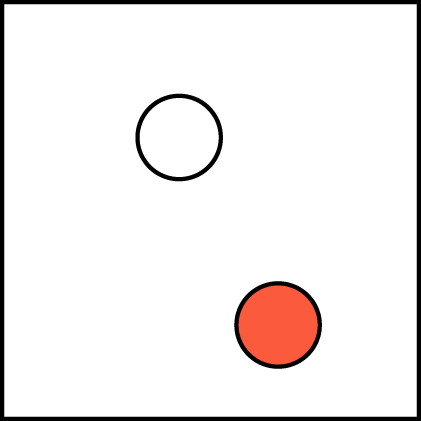
\includegraphics[width=1.5in]{sample}
  \caption{Sample illustration.}
  \label{fig:sampleimage}
\end{figure}

 
\section{Another section}

\section{And yet another section}


\section{Conclusion}

Here is room to sum up your paper and provide an outlook on future developments.
\nocite{*}
%% Do not change the following:
%\bibliographystyle{abbrv}
\printbibliography
\end{document}
